\chapter{Literature Review}
\label{sec:literature_review}

\section{Cell Site Planning}


% terminology:
% Mobile Kommunikation = mobile communications
% Mobilfunk = cellular communications
% Mobilfunknetz = mobile network
% Zellularnetz = cellular network
% Mobilfunkplanung = cellular planning
% Funknetzplanung = radio network planning (RNP)
% Standortplanung = cell site planning

\begin{German}
    \textbf{Mobile Kommunikation} ist ein Teilbereich der Telekommunikation (vgl. \ref{fig:telecommunications_hierarchy}), der sich allgemein mit der drahtlosen Übertragung von Sprache und Daten befasst und sich Empfänger oder Sender frei bewegen können (WLAN, Bluetooth, Satellitenkommunikation, ...) \cite{bundesamtfurstrahlenschutzWhatMobileCommunication}. \textbf{Mobilfunk} ist ein Teilbereich davon, bei dem \textbf{Zellularnetze} verwendet werden \cite{jiangCellularCommunicationNetworks2024}. Ein Zellularnetz setzt sich aus mehreren Funkzellen zusammen. Die Planung dieser Netze wird \textbf{Mobilfunkplanung} genannt. Innerhalb dieses Fachgebiets haben sich wiederum unterschiedliche Disziplinen entwickelt:

    \begin{itemize}
        \item \textbf{Funknetzplanung:} Die Funknetzplanung hat einen elektrotechnischen Fokus und bestimmt, wo Funkzellen stehen sollen, wie das Signal verteilt wird, wie viele Nutzer gleichzeitig verbunden werden können und wie Störungen vermieden werden. \cite{academyforlorawanrAcademyLoRaWANWhat,telecomtrainerRNPRadioNetwork2023}.

        \item \textbf{Standortplanung:} Die Standortplanung hat einen bautechnischen Fokus und bezieht sich auf die Identifikation und bauliche Umsetzung eines physischen Standorts innerhalb des durch die Funknetzplanung definierten Perimeters \cite{habibPDFStudyCell2024}.
    \end{itemize}
\end{German}
    
\begin{English}
    \textbf{Mobile communications} is a subfield of telecommunications (see \ref{fig:telecommunications_hierarchy}) that generally deals with the wireless transmission of voice and data and allows receivers or transmitters to move freely (WLAN, Bluetooth, satellite communication, ...). \cite{bundesamtfurstrahlenschutzWhatMobileCommunication}. \textbf{Cellular communications} is a subfield of this, in which \textbf{cellular networks} are used \cite{jiangCellularCommunicationNetworks2024}. A cellular network consists of several radio cells. The planning of these networks is called \textbf{cellular planning}. Within this field, different disciplines have developed:

    \begin{itemize}
        \item \textbf{Radio Network Planning (RNP):} Radio network planning has an electrical engineering focus and determines where radio cells should be located, how the signal is distributed, how many users can be connected simultaneously, and how interference can be avoided. \cite{academyforlorawanrAcademyLoRaWANWhat,telecomtrainerRNPRadioNetwork2023}.

        \item \textbf{Cell Site Planning:} Cell site planning has a structural engineering focus and refers to the identification and structural implementation of a physical site within the perimeter defined by radio network planning \cite{habibPDFStudyCell2024}.
    \end{itemize}
\end{English}

\begin{figure}[h]
    \centering
    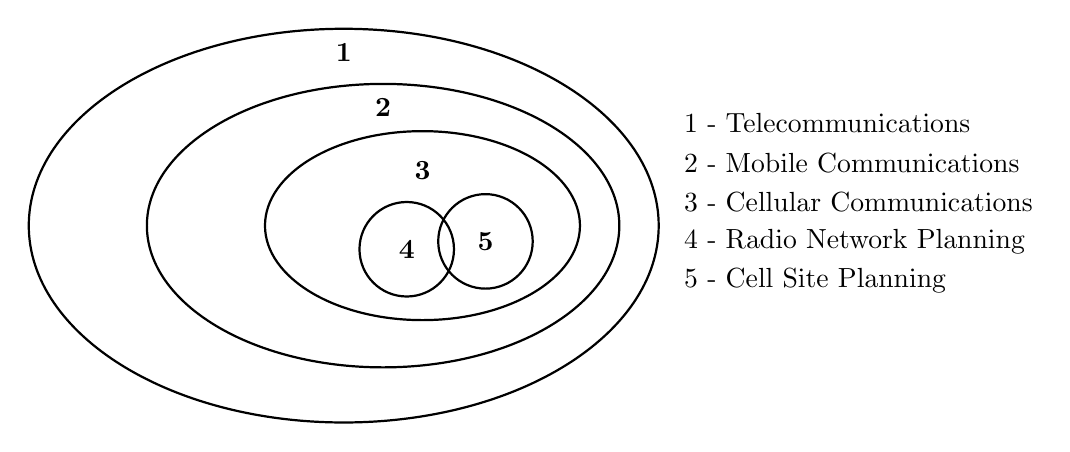
\begin{tikzpicture}
        % Telecommunications (largest ellipse, shifted right)
        \draw[thick] (1,0) ellipse (4 and 2.5);
        \node at (1,2.2) {\textbf{1}}; % Number inside

        % Mobile Communications (subset ellipse, shifted further right)
        \draw[thick] (1.5,0) ellipse (3 and 1.8);
        \node at (1.5,1.5) {\textbf{2}}; % Number inside

        % Cellular Communications (smallest subset ellipse, even further right)
        \draw[thick] (2,0) ellipse (2 and 1.2);
        \node at (2,0.7) {\textbf{3}}; % Number inside

        % Radio Network Planning (small circle inside Cellular Communications)
        \draw[thick] (1.8,-0.3) circle (0.6);
        \node at (1.8,-0.3) {\textbf{4}}; % Number inside

        % Cell Site Planning (small circle inside Cellular Communications)
        \draw[thick] (2.8,-0.2) circle (0.6);
        \node at (2.8,-0.2) {\textbf{5}}; % Number inside

        % Legend (outside the figure)
        \node[right] at (5.2,1.3) {1 - Telecommunications};
        \node[right] at (5.2,0.8) {2 - Mobile Communications};
        \node[right] at (5.2,0.3) {3 - Cellular Communications};
        \node[right] at (5.2,-0.2) {4 - Radio Network Planning};
        \node[right] at (5.2,-0.7) {5 - Cell Site Planning};

    \end{tikzpicture}
    \caption{Telecommunications Hierarchy}
    \label{fig:telecommunications_hierarchy}
\end{figure}


\begin{German}
    Diese Arbeit fokusiert sich auf die Standortplanung. Für die Literaturanalyse wurden zwei allgemeine Werke zu Mobilfunk vom Springer-Verlag \cite{behnkeGrundkursMobilfunkUnd2022,jiangCellularCommunicationNetworks2024} sowie drei unter Standortplanung gelisteten Paper \cite{engelsDimensioningCellSite2013,ahamed5GNetworkCoverage2021,huangAutomaticCellPlanning2000} herangezogen. Es wurde festgestellt, dass hauptsächlich elektrotechnische Themen behandelt werden. Eine mögliche Erklärung könnte sein, dass elektrotechnische Bereiche wie Funktechnik und Signalverarbeitung eine grosse technische Tiefe aufweisen und daher stark erforscht werden. Als Folge wurden dise Bereiche international stark standardisiert (ITU, ETSI, 3GPP). Bauliche Themen hängen dagegen stärker von lokalen Gegebenheiten ab, die durch praxisnahe Richtlinien geregelt werden. Dafür wurde ein vom Bundesrat in Auftrag gegebener Bericht "Nachhaltiges Mobilfunknetz" herangezogen \cite{bundesratNachhaltigesMobilfunknetzBericht2022}.

    Nachfolgend sollen zentrale Erkenntnisse der Literaturanalyse zusammengefasst werden. Im Bereich der Standortplanung wird auf die Terminologie der Schweizer Mobilfunkbrache zurückgegriffen.
\end{German}

\begin{English}
    This work focuses on cell site planning. For the literature analysis, two general works on mobile communications from Springer \cite{behnkeGrundkursMobilfunkUnd2022,jiangCellularCommunicationNetworks2024} as well as three papers listed under cell site planning \cite{engelsDimensioningCellSite2013,ahamed5GNetworkCoverage2021,huangAutomaticCellPlanning2000} were consulted. It was found that mainly electrical engineering topics are addressed. One possible explanation could be that electrical engineering areas such as radio technology and signal processing have a high technical depth and are therefore extensively researched. As a result, these areas have been strongly standardized internationally (ITU, ETSI, 3GPP). Structural topics, on the other hand, depend more on local conditions, which are regulated by practical guidelines. For this purpose, a report commissioned by the Federal Council "Sustainable Mobile Network" was consulted \cite{bundesratNachhaltigesMobilfunknetzBericht2022}.

    The following section summarizes key findings of the literature analysis. In the field of cell site planning, the terminology of the Swiss mobile communications industry is used.
\end{English}


\subsection{International Status}
\begin{German}
    Der gesamte mobile Datenverkehr nimmt weltweit exponentiell zu \cite{EricssonMobilityReport}. Bis ungefähr 2020 verdoppelte sich der Verkehr etwa alle zwei Jahre. Für die Zeit bis 2030 werden noch immer jährliche Wachstumsraten von durchschnittlich 19 \% prognostiziert. Derzeit werden 34 \% des mobilen Datenverkehrs über 5G-Netzwerke abgewickelt. Bis 2030 soll dieser Anteil auf 80 \% steigen.

    Zum Anstieg entscheidend beigetragen haben Video-Streaming mit immer höheren Bildschirmauflösungen (4K, 8K), das mitlerweile 74 \% des mobilen Datenverkehrs ausmacht \cite{EricssonMobilityReport}. Haupttreiber des zukünftigen Wachstums wird besonders in den Bereichen des autonomen Fahren, Extended Reality, Industrie 4.0 sowie generativer KI gesehen. 
    Fixed Wireless Access (FWA) wird stark an bedeutung gewinnen und bis 2030 mit 36 \% einen erheblichen Anteil des Datenverkehrs ausmachen. Dabei werden stationäre Geräte (z. B. Computer) über ein CPE-Gerät mit einer festen Breitbandverbindung versorgt, die über mobile Netzwerke (4G/5G) bereitgestellt wird. Besonders in wirtschaftlich schwächer entwickelten Regionen wird FWA traditionelle Festnetzanschlüsse zunehmend als kostengünstigere Alternative verdrängen. 
\end{German}

\begin{English}
    Worldwide, mobile data traffic is increasing exponentially \cite{EricssonMobilityReport}. Until around 2020, traffic doubled about every two years. Annual growth rates of an average of 19 \% are still forecast for the period until 2030. Currently, 34 \% of mobile data traffic is handled via 5G networks. By 2030, this share is expected to increase to 80 \%.

    The increase has been significantly driven by video streaming with ever higher screen resolutions (4K, 8K), which now accounts for 74 \% of mobile data traffic \cite{EricssonMobilityReport}. The main drivers of future growth are seen particularly in the areas of autonomous driving, Extended Reality, Industry 4.0, and generative AI. 
    Fixed Wireless Access (FWA) will become increasingly important and account for a significant share of the traffic by 2030 with 36 \%. Stationary devices (e.g., computers) are supplied with a fixed broadband connection via a CPE device provided by mobile networks (4G/5G). Especially in economically less developed regions, FWA will increasingly displace traditional fixed network connections as a more cost-effective alternative.
\end{English}

\subsection{National Status}
\begin{German}
    In der Schweiz vertritt der Bund die Ansicht, dass eine leistungsfähige Telekommunikationsinfrastruktur für die Wirtschaft und Gesellschaft einen hohen Stellenwert hat \cite{bundesratNachhaltigesMobilfunknetzBericht2022}. Ein rascher Ausbau leistungsfähriger 5G Netze sei deshalb wichtig. Nach Angaben der Betreiber Swisscom, Sunrise und Salt sind dafür 7'500 neue Antennenstandorte und Investitionen in der Höhe von 3.2 Milliarden Franken notwendig \cite{bundesratNachhaltigesMobilfunknetzBericht2022}. Die drei Anbieter betreiben zusammen knapp 20'000 Standorte \cite{federalofficeofcommunicationsofcomLocationsMobilePhone}. Ihr Marktanteil nach Kundenanzahl lag Ende 2023 bei Swisscom 54.3 \%, bei Sunrise 23.6 \% und bei Salt 17.1 \% \cite{bakomMarktanteileMobilfunknetz}. Die Marktdurchdringung betrug 128.9 \%. Damit gibt es mehr aktive Simkarten als Einwohner \cite{bakomAnzahlMobilfunkkundinnenUnd}.

    Zum Schutz der Bevölkerung vor wissenschaftlich nachgeweisenen Schäden aufgrund nichtionisierender Strahlung (NIS), hat die International Commission on Non-Ionizing Radiation Protection (ICNIRP) empfohlene Grenzwerte definiert \cite{baumannMitVerordnungUeber2005}. Diese wurden vom Bund in der Verordnung über den Schutz vor nichtionisierender Strahlung (NISV) als Immissionsgrenzwerte übernommen und entsprechen der Empfehlung der EU. Diese müssen an allen Orten eingehalten werden, an denen sich Menschen aufhalten können. Aufgrund gesundheitlicher Bedenken, wurden sogenannte Anlagegrenzwerte definiert. Dieser verschärfte Grenzwert beträgt noch 10 \% des Immissionsgrenzwert und muss an Orten mit empfindlicher Nutzung (OMEN) eingehalten werden. Dies sind Bereiche, von denen auszugehen ist, dass sich Menschen regelmässig über längere Zeit aufhalten. Die elektrische Feldstärke beträgt dort ein Zehntel des in Deutschland und Frankreich zulässigen Wertes. Die Leistung einer elektromagnetischen Welle ist dabei proprtional zum Quadrat der elektrischen Feldstärke. Eine um Faktor 10 reduzierte Feldstärke, führt damit zu einer um Faktor 100 sinkenden Sendeleistung \cite{chance5gAnlagegrenzwerteImMobilfunk}.
    Sobald eine Anlage die maximal zulässige Sendeleistung erreicht hat, kann diese nicht mehr weiter ausgebaut werden. Zur Erhöhung der Netzkapazität müssen dann neue Stanorte gebaut werden. \cite{bundesratNachhaltigesMobilfunknetzBericht2022}
\end{German}

\begin{English}
    In Switzerland, the federal government is of the opinion that a powerful telecommunications infrastructure is of high importance for the economy and society \cite{bundesratNachhaltigesMobilfunknetzBericht2022}. Therefore, a rapid expansion of powerful 5G networks is important. According to the operators Swisscom, Sunrise, and Salt, 7,500 new antenna sites and investments of CHF 3.2 billion are required for this \cite{bundesratNachhaltigesMobilfunknetzBericht2022}. The three providers together operate almost 20,000 sites \cite{federalofficeofcommunicationsofcomLocationsMobilePhone}. Their market share by number of customers was 54.3 \% for Swisscom, 23.6 \% for Sunrise, and 17.1 \% for Salt at the end of 2023 \cite{bakomMarktanteileMobilfunknetz}. The market penetration was 128.9 \%. This means that there are more active SIM cards than inhabitants \cite{bakomAnzahlMobilfunkkundinnenUnd}.

    To protect the population from scientifically proven damage due to non-ionizing radiation (NIS), the International Commission on Non-Ionizing Radiation Protection (ICNIRP) has defined recommended limit values \cite{baumannMitVerordnungUeber2005}. These were adopted by the federal government in the Ordinance on Protection against Non-Ionizing Radiation (NISV) as immission limit values and correspond to the EU recommendation. These must be complied with at all locations where people can stay. Due to health concerns, so-called system limit values were defined. This stricter limit value is 10 \% of the immission limit value and must be complied with at locations with sensitive use (OMEN). These are areas where it is assumed that people stay regularly for longer periods. The electric field strength there is one-tenth of the permissible value in Germany and France. The power of an electromagnetic wave is proportional to the square of the electric field strength. A field strength reduced by a factor of 10 thus leads to a transmission power reduced by a factor of 100 \cite{chance5gAnlagegrenzwerteImMobilfunk}.
\end{English}

\subsection{Cellular Network Generations}

% terminology:
% Generation = Generation
% Mobilfunkgeneration = Cellular network generation

\begin{German}
    Ungefähr alle zehn Jahre wird eine neue Mobilfunkgeneration eingeführt \cite{bundesratNachhaltigesMobilfunknetzBericht2022}. Diese haben jeweils eine höhere Datenübertragungsrate, eine geringere Latenz und eine höhere Anzahl an gleichzeitig verbundenen Geräten. Bis zur Einführung der sechten Generation (6G Vision) ca. 2030 wird derzeit die fünfte Generation (5G) ausgebaut. Ebenfalls praxisrelevant ist die vierte Generation (LTE), die ab 2012 ausgebaut wurde. Die dritte Generation (UMTS) wird als erstes von Swisscom auf Ende 2025 eingestellt \cite{swisscomAbschaltung3GErneuerung}. Die zweite Generation (GSM) wurde von den drei Anbeitern zwischen 2021 und 2023 eingestellt \cite{onlineSchweizEndgueltigesAus2022}.
\end{German}

\begin{English}
    Approximately every ten years, a new cellular network generation is introduced \cite{bundesratNachhaltigesMobilfunknetzBericht2022}. Each of these has a higher data transmission rate, lower latency, and a higher number of devices connected simultaneously. Until the introduction of the sixth generation (6G Vision) around 2030, the fifth generation (5G) is currently being expanded. Also practically relevant is the fourth generation (LTE), which was expanded from 2012. The third generation (UMTS) will be discontinued by Swisscom by the end of 2025 \cite{swisscomAbschaltung3GErneuerung}. The second generation (GSM) was discontinued by the three providers between 2021 and 2023 \cite{onlineSchweizEndgueltigesAus2022}.
\end{English}

\subsection{Network Architecture}

% terminology:
% Netzarchitektur = Network architecture
% Zugangsnetz = Access network
% Kernnetz = Core network
% Backhaul-Anbindung = Backhaul connection
% Ständermast = Stand-Mounted Pole
% Fassadenmast = Wall-Mounted Pole
% Dachstockmast = Attic-Mounted Pole
% Funkzelle = Radio cell

\begin{German}
    Die Netzarchitektur eines Mobilfunknetzes kann in verschiedene Komponenten gegliedert werden \cite{behnkeGrundkursMobilfunkUnd2022,jiangCellularCommunicationNetworks2024}:

    \begin{itemize}
        \item \textbf{Zugangsnetz:} Das Zugangsnetz empfängt Signale vom Endgerät (z. B. Smartphone) und leitet sie an das Kernnetz weiter. Es umfasst die Endgeräte, die Sendeanlagen und die Funkverbindung zwischen ihnen. 
        \item \textbf{Kernnetz:} Das Kernnetz verarbeitet, steuert und vermittelt die Verbindungen und ermöglicht die Anbindung an externe Netze, wie das Internet oder das Festnetz. Jeder Betreiber hat sein eigenes Kernnetz.
        \item \textbf{Backhaul-Anbindung:} Die beiden Netze sind über die Backhaul-Anbindung verbunden, die aufgrund ihrer hohen Kapazität vorzugsweise leitungsbasiert über Glasfaser realisiert wird. In abgelegenen Gebieten kann sie jedoch auch als Richtfunkverbindung umgesetzt werden.
    \end{itemize}

    Herzstück jeder Anlage ist die \textbf{Basisstation}, die zentrale Recheneinheit zur Steuerung der Datenübertragung.  Jede Basisstation besitz zudem mindestens eine \textbf{Antenne}, über die mittels elektromagnetischen Wellen eine bidirektionale Kommunikation mit dem Endgerät erfolgt. Üblicherweise werden pro Analge drei Sektor-Antennen verwendet, die jeweils gerichtet in einen Sektor von 120 Grad abstrahlen. Bei unterschiedlichen Technologien werden diese in unterschiedlichen Ebenen angeordnet. Jeder Antennensektor definiert dabei eine \textbf{Funkzelle}. Dadurch ergibt sich ein idealisiertes, sechseckiges Grundmuster. \cite{behnkeGrundkursMobilfunkUnd2022}
\end{German}

\begin{English}
    The network architecture of a cellular network can be divided into various components \cite{behnkeGrundkursMobilfunkUnd2022,jiangCellularCommunicationNetworks2024}:

    \begin{itemize}
        \item \textbf{Access network:} The access network receives signals from the end device (e.g., smartphone) and forwards them to the core network. It includes the end devices, the transmitting systems, and the radio connection between them.
        \item \textbf{Core network:} The core network processes, controls, and mediates the connections and enables connections to external networks such as the Internet or the fixed network. Each operator has its own core network.
        \item \textbf{Backhaul connection:} The two networks are connected via the backhaul connection, which is preferably implemented as a line-based connection via fiber optic due to its high capacity. However, in remote areas, it can also be implemented as a microwave connection.
    \end{itemize}

    The \textbf{base station} is the central processing unit for controlling data transmission and is the heart of each system. Each base station also has at least one \textbf{antenna} through which bidirectional communication with the end device takes place via electromagnetic waves. Typically, three sector antennas are used per system, each radiating in a sector of 120 degrees. These are arranged in different planes for different technologies. Each antenna sector defines a \textbf{radio cell}. This results in an idealized hexagonal basic pattern. \cite{behnkeGrundkursMobilfunkUnd2022}
\end{English}

\subsection{Site Classification}
\begin{German}
    Während in der Funknetzplanung die Klassifizierung nach Zellgrösse (Makrozellen, Mikrozellen, Pikozellen, Femtozellen) üblich ist \cite{jiangCellularCommunicationNetworks2024}, hat sich in der schweizerischen Standortplanung folgende Unterteilung (vgl. \ref{fig:site_classification}) etabliert: 

    \begin{itemize}
        \item \textbf{Greenfield-Standort:} Dieser Standorttyp ist überwiegen in ländlichen Gebieten anzutreffen Charakteristisch dafür ist ein üblicherweise zwischen 20 und 50 Meter hocher, freistehender Mast.
        \item \textbf{Rooftop-Standort:} Dieser Standorttyp ist überwiegen in besiedelten Gebieten anzutreffen. Charakteristisch dafür ist die Unterbringung auf dem Dach eines bestehenden Gebäudes. Je nach gewählter Mastkonstruktion kann weiter unterschieden werden:
        \begin{itemize}
            \item \textbf{Ständerkonstruktion [2]:} Mit dem Gebäude nicht fest verbundener Mast, der auf eine Stahlunterkonstruktion aufgesetzt wird und auf dem Dach platziert wird.
            \item \textbf{Fassadenmast [3]:} Mit dem Gebäude fest verbundener Mast, der an der Fassade montiert wird. 
            \item \textbf{Dachstockmast [4]:} Mit dem Gebäude fest verbundener Mast, der im Gebäudeinnern montiert wird und durch eine Öffnung im Dach ins Freie ragt.
        \end{itemize}
    \end{itemize}
\end{German}

\begin{English}
    While in radio network planning the classification by cell size (macrocells, microcells, picocells, femtocells) is common \cite{jiangCellularCommunicationNetworks2024}, the following classification (see \ref{fig:site_classification}) has established itself in Swiss site planning:

    \begin{itemize}
        \item \textbf{Greenfield site:} This type of site is mainly found in rural areas. Characteristic of this is a usually between 20 and 50 meters high, freestanding mast.
        \item \textbf{Rooftop site:} This type of site is mainly found in populated areas. Characteristic of this is the placement on the roof of an existing building. Depending on the chosen mast construction, further distinctions can be made:
        \begin{itemize}
            \item \textbf{Stand-mounted pole [2]:} Mast not firmly connected to the building, which is placed on a steel substructure and placed on the roof.
            \item \textbf{Wall-mounted pole [3]:} Mast firmly connected to the building, which is mounted on the facade.
            \item \textbf{Attic-mounted pole [4]:} Mast firmly connected to the building, which is mounted inside the building and protrudes through an opening in the roof to the outside.
        \end{itemize}
    \end{itemize}
\end{English}

\begin{figure}[h]
    \centering
    \includegraphics[width=1\textwidth]{dwg/site_classification.PNG}
    \caption{Site Classification}
    \label{fig:site_classification}
\end{figure}

\section{Building Information Modeling (BIM)}
\begin{German} 
    \textbf{Building Information Modeling (BIM)} ist in erster Linie eine Methodik zur digitalen Planung, Ausführung und Verwaltung von Bauwerken über den gesamten Lebenszyklus hinweg \cite{astourLehrbuchGrundlagenBIMArbeitsmethode2022}. In der Praxis wird BIM daher häufig als Synonym für eine modellbasierte Planung verwednet, obschon BIM über die reine 3D-Modellierung hinaus gehen kann (z.B. 4D). Zur präzisen Abgrenzung zum Werkzeug, dass diese Methodik ermöglicht, wird dieses nachfolgend \textbf{BIM-Software} genannt.

    Für die Literaturanalyse wurden die beiden Fachbücher \cite{astourLehrbuchGrundlagenBIMArbeitsmethode2022,mayBIMImImmobilienbetrieb2022} herangezogen. Aufgrund ihres umfassenden Inhalts wurde auf die Konsultation weiterer wissenschaftlicher Publikationen verzichtet. Nachfolgend sollen zentrale Erkenntnisse der Literaturanalyse zusammengefasst werden.
\end{German}

\begin{English}
    \textbf{Building Information Modeling (BIM)} is primarily a methodology for digitally planning, executing, and managing buildings over the entire life cycle \cite{astourLehrbuchGrundlagenBIMArbeitsmethode2022}. In practice, BIM is therefore often used as a synonym for model-based planning, although BIM can go beyond mere 3D modeling (e.g., 4D). To clearly distinguish it from the tool that enables this methodology, it will be referred to as \textbf{BIM software} below.

    For the literature analysis, the two textbooks \cite{astourLehrbuchGrundlagenBIMArbeitsmethode2022,mayBIMImImmobilienbetrieb2022} were consulted. Due to their comprehensive content, further scientific publications were not consulted. The following section summarizes key findings of the literature analysis.
\end{English}

\subsection{Characteristics of a BIM Model}
\begin{German}
    Ein \textbf{BIM-Modell} besteht zunächst, wie das dreidimensionale \textbf{CAD-Modell} auch, aus geometrischen Daten im dreidimensionalen Raum. Zusätzlich zu den geometrischen Daten enthält das BIM-Modell jedoch weitere Informationen, die als \textbf{Attribute} bezeichnet werden. Während das CAD-Modell eine Aggregation rein geometrischer Primitive (Punkte, Linien, Flächen) darstellt, besteht das BIM-Modell aus parametrisierten Objekten. Dabei handelt es sich um intelligente \textbf{Bauteile}, die neben ihrer Geometrie auch Attribute wie Material und Kosten enthalten können. Diese Informationen müssen im CAD-Modell entweder graphisch oder textuell dargestellt werden. Zudem können Bauteile semantisch verknüpft werden, um Beziehungen zu modellieren. Dies soll an folgendem Beispiel dargestellt werden. \cite{astourLehrbuchGrundlagenBIMArbeitsmethode2022} \\
    
    \begin{itshape}
    \textbf{Beispiel Ingenieurbau}\\
    Eine Decke eines Einfamilienhauses soll um 10 cm abgesenkt werden.

    \textbf{BIM}: Im BIM-Modell wird das Bauteil \texttt{Decke} abgesenkt. Die Änderung wird automatisch in den Schal- und Bewehrungsplänen abgebildet. Die Bewehrungsliste wird automatisch aktualisiert. Die finanziellen Auswirkungen können direkt über eine Kostenberechnung ermittelt werden.

    \textbf{CAD \footnote{Moderne CAD-Systeme verfügen mittlerweile auch über halbautomatisierte Funktionen.}}: Die Decke wird im CAD-Modell abgesenkt. Die Änderung wird manuell in den Schal- und Bewehrungsplänen übertragen. Die Bew
    ehrungsliste muss manuell aktualisiert werden. Die finanziellen Auswirkungen müssen separat berechnet werden.
    \end{itshape}
\end{German}

\begin{English}
    A \textbf{BIM model} initially consists, like the three-dimensional \textbf{CAD model}, of geometric data in three-dimensional space. In addition to the geometric data, however, the BIM model contains additional information, referred to as \textbf{attributes}. While the CAD model represents an aggregation of purely geometric primitives (points, lines, surfaces), the BIM model consists of parametrized objects. These are intelligent \textbf{components} that can contain attributes such as material and costs in addition to their geometry. This information must be represented graphically or textually in the CAD model. In addition, components can be semantically linked to model relationships. This will be illustrated by the following example. \cite{astourLehrbuchGrundlagenBIMArbeitsmethode2022} \\

    \begin{itshape}
    \textbf{Example Civil Engineering}\\
    A ceiling slab of a single-family house is to be lowered by 10 cm.

    \textbf{BIM}: The component \texttt{ceiling slab} is lowered in the BIM model. The change is automatically reflected in the formwork and reinforcement plans. The reinforcement list is updated automatically. The financial implications can be determined directly via a cost calculation.

    \textbf{CAD \footnote{Modern CAD systems now also have semi-automated functions.}}: The ceiling slab is lowered in the CAD model. The change is manually transferred to the formwork and reinforcement plans. The reinforcement list must be updated manually. The financial implications must be calculated separately.
    \end{itshape}
 

\end{English}

\subsection{BIM Terminology}
\begin{German}
    Zur Bewertung und Klassifizierung von BIM-Prozessen und BIM-Modellen gibt es standardisierte Kennzahlen. Diese ermöglichen eine objektive Bewertung und erleichtern die Kommunikation zwischen den Projektbeteiligten. Die wichtigsten Kennzahlen sind:
\end{German}

\begin{English}
    Standardized metrics are available for evaluating and classifying BIM processes and BIM models. These enable an objective evaluation and facilitate communication between project participants. The most important metrics are:
\end{English}

\subsubsection{BIM Maturity Level}
\begin{German}
    Der \textbf{BIM-Reifegrad} ist ein Qualitätsmass, das beschreibt, wie systematisch und umfassend BIM in einem Unternehmen oder Projekt implementiert ist. Der Schwerpunkt liegt auf der Vernetzung von Daten, der Standardisierung sowie der Zusammenarbeit zwischen den Beteiligten. Gemäß VDI 2552 werden die folgenden vier Reifegrade unterschieden: \cite{astourLehrbuchGrundlagenBIMArbeitsmethode2022,eichlerBIMcertHandbuchGrundlagenwissen2023}\\
\end{German}
\begin{English}
    The \textbf{BIM maturity level} is a quality measure that describes how systematically and comprehensively BIM is implemented in a company or project. The focus is on data networking, standardization, and collaboration between the participants. According to VDI 2552, the following four maturity levels are distinguished: \cite{astourLehrbuchGrundlagenBIMArbeitsmethode2022,eichlerBIMcertHandbuchGrundlagenwissen2023}\\
\end{English}

\begin{table}[h]
    \centering
    \renewcommand{\arraystretch}{1.2} % Adjust row height for better readability
    \setlength{\tabcolsep}{5pt} % Adjust column spacing
    \begin{tabularx}{\textwidth}{|c|l|X|}
        \hline
        \textbf{Level} & \textbf{BIM Usage} & \textbf{Description}  \\
        \hline
        \textbf{0} & None &  Traditional 2D CAD drafting is used with no object-based modeling or intelligent data sharing. Collaboration is minimal, and document exchange is paper-based or in simple file formats. \\
        \hline
        \textbf{1} & None &  Combination of 2D and 3D CAD tools. While 3D models may be used internally, there is no standardized collaboration between different disciplines. Data exchange remains file-based without integrated workflows. \\
        \hline
        \textbf{2} & Collaborative &  Different disciplines work on their own BIM models, which are then shared and combined at specific project stages. Collaboration is structured, but data exchange is still semi-automated, requiring manual coordination. Lifecycle phases are considered separately. \\
        \hline
        \textbf{3} & Integrated & All disciplines collaborate in a fully connected and shared BIM environment. A single, integrated model covers the entire building lifecycle, from design to operation. Automated data exchange and real-time collaboration enable seamless workflows. \\
        \hline
    \end{tabularx}
    \caption{BIM Stages and Their Characteristics}
    \label{tab:BIM_stages}
\end{table}

\subsubsection{Level of Development (LOD)}

\begin{German}
    Der \textbf{Fertigstellungsgrad (LOD)} eines Modells gibt an, wie viele Projektinformationen bereits im Modell enthalten sind. Dieser setzt sich zusammen aus dem Ausarbeitungsgrad der Geometrie (LOG) und der Tiefe der alphanumerischen Information (LOI):  \\
\end{German}
\begin{English}
    The \textbf{level of development (LOD)} of a model indicates how much project information is already contained in the model. This consists of the degree of elaboration of the geometry (LOG) and the depth of the alphanumeric information (LOI):  \\
\end{English}

    \begin{equation}
        \text{LOD} = \text{LOG} + \text{LOI}
    \end{equation}
    
 \begin{German}   
    Der LOD gibt somit den Fertigstellungsgrad eines Modells zu einer bestimmten Projektphase an. Dieser wird mit Zahlen zwischen 100 und 500 gekennzeichnet (vgl. \ref{fig:Level_of_Development}). Dabei nimmt der Detailierungsgrad mit steigender Zahl zu. Mit fortschreitendem Planungsstand nimmt der LOD in der Regel zu. Da ein hoher LOD mit einem höheren Arbeitsaufwand verbunden ist, ist es wichtig zu bestimmen, wie viele Details zu welchem Zeitpunkt sinvoll sind. Dies wird mit dem Level of Information Need (LOIN) angegeben. \cite{astourLehrbuchGrundlagenBIMArbeitsmethode2022}
\end{German}
\begin{English}
    The LOD thus indicates the level of completion of a model at a specific project phase. This is marked with numbers between 100 and 500 (see \ref{fig:Level_of_Development}). The level of detail increases with increasing number. As the planning progresses, the LOD usually increases. Since a high LOD is associated with a higher workload, it is important to determine how many details are useful at what time. This is indicated by the Level of Information Need (LOIN). \cite{astourLehrbuchGrundlagenBIMArbeitsmethode2022}
\end{English}

    % Insert a picture
    \begin{figure}[h]
        \centering
        \includegraphics[width=1\textwidth]{images/bim_levels_of_development.png}
        \caption{Level of Development (LOD) \cite{ncircletechBIMLevelDevelopment}}
        \label{fig:Level_of_Development}
    \end{figure}

\subsubsection{BIM Dimensions}
\begin{German}
    Die \textbf{BIM-Dimension} beschreibt die Informationstiefe der Attribute. Sie wird angegeben durch einen Wert zwischen 3D bis 7D. Dabei nimmt der Detailierungsgrad mit steigender Zahl zu. \cite{mayBIMImImmobilienbetrieb2022}
\end{German}
\begin{English}
    The \textbf{BIM dimension} describes the depth of information of the attributes. It is indicated by a value between 3D and 7D. The level of detail increases with increasing number. \cite{mayBIMImImmobilienbetrieb2022}
\end{English}

% table
\begin{table}[h]
    \centering
    \renewcommand{\arraystretch}{1.2} % Adjust row height for better readability
    \setlength{\tabcolsep}{5pt} % Adjust column spacing
    \resizebox{\textwidth}{!}{ % Resizes table to fit within text width
    \begin{tabular}{|c|l|l|}
        \hline
        \textbf{Dimension} & \textbf{Additional Attributes} & \textbf{Use Cases} \\
        \hline
        \textbf{3D} & None & Geometric modeling \\
        \hline
        \textbf{4D} & Time & Construction scheduling, project phases \\
        \hline
        \textbf{5D} & Cost & Quantity takeoff, pricing, budgeting \\
        \hline
        \textbf{6D} & Efficiency \& Sustainability & Energy performance, lifecycle assessment \\
        \hline
        \textbf{7D} & Facility management & Operations, maintenance, asset tracking \\
        \hline
    \end{tabular}
    }
    \caption{BIM Dimensions and Information Depth}
    \label{tab:BIM_dimensions}
\end{table}

\subsubsection{BIM Types}
\begin{German}
    BIM-Anwendungsformen werden in der Ausprägung hinsichtlich zwier Dimensionen unterschieden: \cite{astourLehrbuchGrundlagenBIMArbeitsmethode2022}
    
    \begin{enumerate}
        \item \textbf{Eingriffstiefe:} Quantitätsmass, das beschreibt, inwieweit ein BIM-Modell in die Wertschöpfungskette integriert ist. Eine geringe Eingriffstiefe liegt vor, wenn BIM nur in einer einzelnen Phase genutzt wird. Eine hohe Eingriffstiefe bedeutet, dass BIM über den gesamten Lebenszyklus hinweg eingesetzt wird.
        \item \textbf{Herstellerunabhängigkeit:} Qualitätsmass der Interoperabilität, also der Fähigkeit, BIM-Modelle und Daten ausserhalb von bestimmten Softwarefamilien oder Anbietern zu nutzen.
    \end{enumerate}

    Durch die Ausprägung der beiden Dimensionen ergeben sich die folgenden vier BIM-Typen: 
\end{German}

\begin{English}
    BIM application forms are distinguished in terms of two dimensions: \cite{astourLehrbuchGrundlagenBIMArbeitsmethode2022}
    
    \begin{enumerate}
        \item \textbf{Depth of Integration:} Quantity measure that describes the extent to which a BIM model is integrated into the value chain. A low depth of integration exists when BIM is only used in a single phase. A high depth of integration means that BIM is used throughout the entire life cycle.
        \item \textbf{Software Independence:} Quality measure of interoperability, i.e., the ability to use BIM models and data outside of specific software families or providers.
    \end{enumerate}

    The following four BIM types result from the expression of the two dimensions:
\end{English}

\begin{figure}[h]
    \centering
    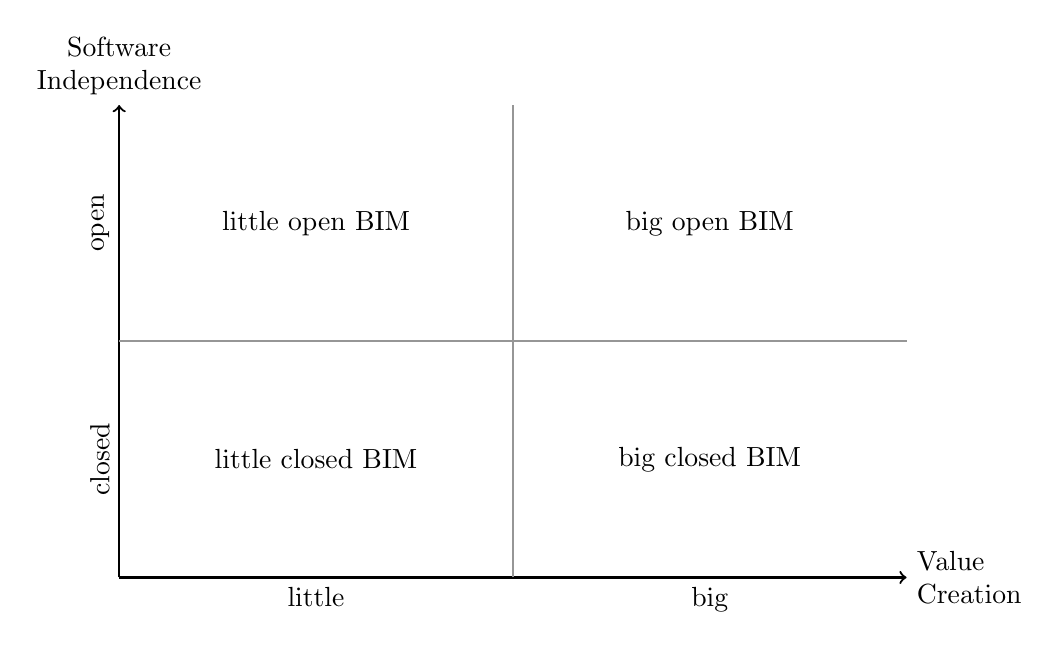
\begin{tikzpicture}

        % Define Axis Styles
        \draw[thick,->] (0,0) -- (10,0) node[anchor=west, align=left] {Value \\ Creation};
        \draw[thick,->] (0,0) -- (0,6) node[anchor=south, align=center] {Software \\ Independence};
        \node[anchor=north] at (2.5,0) {little};
        \node[anchor=north] at (7.5,0) {big};
        \node[anchor=south, rotate=90] at (0,1.5) {closed};
        \node[anchor=south, rotate=90] at (0,4.5) {open};

        % Draw Quadrant Lines
        \draw[thick, color={rgb,255:red,150; green,150; blue,150}] (5,0) -- (5,6); % Vertical
        \draw[thick, color={rgb,255:red,150; green,150; blue,150}] (0,3) -- (10,3); % Horizontal

        % Labels for quadrants
        \node at (2.5,4.5) {little open BIM};
        \node at (7.5,4.5) {big open BIM};
        \node at (2.5,1.5) {little closed BIM};
        \node at (7.5,1.5) {big closed BIM};

    \end{tikzpicture}
    \caption{BIM Types}
\end{figure}

\subsection{BIM Management}
\begin{German}
    Das \textbf{BIM-Management} beinhaltet die strategische und operative Steuerung von BIM. Es sollen damit Workflows standardisiert und die Zusammenarbeit verbessert werden. In diesem Unterkapitel sollen drei Werkzeuge vorgestellt werden (vgl. \ref{fig:BIM_management}), auf die in der Fallstudie zurückgegriffen wird.
\end{German}
\begin{English}
    \textbf{BIM management} involves the strategic and operational control of BIM. The aim is to standardize workflows and improve collaboration. In this subchapter, three tools will be presented (see \ref{fig:BIM_management}), which will be used in the case study.
\end{English}

\subsubsection{Exchange Information Requirements (EIR)}
\begin{German}
    Die \textbf{Auftraggeber-Informations-Anforderungen (AIA)} entsprechen einem auf BIM zugeschnittenen Lastenheft. Sie beschreiben, warum welche Information wann benötigt werden. Sie definieren die Anforderungen des Auftraggebers an BIM-Prozesse, Daten und Zusammenarbeit über den gesamten Projektlebenszyklus. Dazu gehören Vorgaben zu Modellstruktur, Detaillierungsgrad, Datenaustauschformaten, Verantwortlichkeiten und Kollaborationsmethoden. \cite{astourLehrbuchGrundlagenBIMArbeitsmethode2022}
\end{German}
\begin{English}
    The \textbf{Exchange Information Requirements (EIR)} correspond to a specification tailored to BIM. They describe why which information is needed when. They define the client's requirements for BIM processes, data, and collaboration throughout the entire project life cycle. This includes specifications for model structure, level of detail, data exchange formats, responsibilities, and collaboration methods. \cite{astourLehrbuchGrundlagenBIMArbeitsmethode2022}
\end{English}

\subsubsection{BIM Execution Plan (BEP)}
\begin{German}
    Der \textbf{BIM-Abwicklungsplan (BAP)} entspricht einem auf BIM zugeschnittenen Pflichtenheft. Er beschreibt, wie die Anforderungen aus dem \textbf{Auftraggeber-Informations-Anforderungen (AIA)} vom Auftragnehmer im Projekt umgesetzt werden. \cite{astourLehrbuchGrundlagenBIMArbeitsmethode2022}
\end{German}
\begin{English}
    The \textbf{BIM Execution Plan (BEP)} corresponds to a specification tailored to BIM. It describes how the requirements from the \textbf{Employer's Information Requirements (EIR)} are implemented by the contractor in the project. \cite{astourLehrbuchGrundlagenBIMArbeitsmethode2022}
\end{English}

\subsubsection{BIM Modeling Guidelines}
\begin{German}
    Die \textbf{BIM-Modellierungsrichtlinien} legen fest, wie ein BIM-Modell aufgebaut und strukturiert sein soll. Dafür werden Standards, Methoden und Anforderungen für die Erstellung und Verwaltung definiert. Sie sorgen für einheitliche Datenstrukturen, bessere Zusammenarbeit und eine hohe Modellqualität. Typischerweise werden die Modelleriungsrichtlinien im BAP definiert oder referenziert. \cite{astourLehrbuchGrundlagenBIMArbeitsmethode2022}
\end{German}
\begin{English}
    The \textbf{BIM modeling guidelines} define how a BIM model should be structured and organized. For this purpose, standards, methods, and requirements for creation and management are defined. They ensure uniform data structures, better collaboration, and high model quality. Typically, the modeling guidelines are defined or referenced in the BEP. \cite{astourLehrbuchGrundlagenBIMArbeitsmethode2022}
\end{English}

\begin{figure}[h]
    \centering
    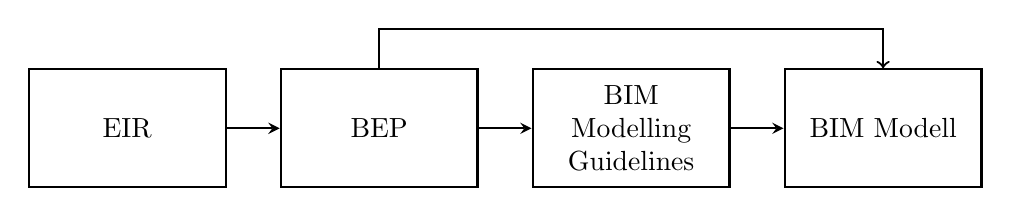
\begin{tikzpicture}[
        node distance=3.2cm, % Distance between nodes
        every node/.style={draw, minimum width=2.5cm, minimum height=1.5cm, align=center}, % Box styling
        every path/.style={thick, -stealth} % Arrow styling
        ]
        
        % Define nodes
        \node (EIR) {EIR};
        \node (BEP) [right of=EIR] {BEP};
        \node (Modelling) [right of=BEP] {BIM \\ Modelling \\ Guidelines};
        \node (BIM) [right of=Modelling] {BIM Modell};

        % Draw arrows
        \draw (EIR) -- (BEP);
        \draw (BEP) -- (Modelling);
        \draw (Modelling) -- (BIM);
        
        % Draw additional curved arrow from EIR to BIM Modell
        \draw[->] (BEP.north) |- ([yshift=0.5cm] BIM.north) -| (BIM.north);

    \end{tikzpicture}
    \caption{Simplified BIM Management Process Flow}
    \label {fig:BIM_management}
\end{figure}

\section{Scan-to-BIM}
\begin{German}
    Umbauprojekte werden in der Schweizer Bauwirtschaft immer wichtiger. Die Bauausgaben für Neubauten sind gegenüber 1980 beinahe gleich geblieben. Die Investitionen in Umbauten, Erweiterungen und Abbrüche hat sich in der gleichen Periode über verdreifacht \cite{bundesamtfuerstatstikBauausgabenNachArt}. Damit betragen die gesamtschweizerischen Investitionen für Umbauten, Erweiterungen und Abbrüchen bereits 66 \% jener für Neubauten. 

    Gleichzeitig ist bei privaten Bestandsbauten die Dokumentation häufig lückenhaft \cite{dewolfCircularBuiltEnvironmentg, kadenLeitfadenGeodaesieUnd}. Besonders ältere Gebäude verfügen oft nur über unvollständige oder veraltete Planunterlagen. Zwar lassen sich in Gemeindearchiven häufig Baueingabepläne auffinden, diese dokumentieren jedoch den ursprünglichen Bauzustand, sind oft überholt und in niedrigem Detailierungsgrad.
    
    In der Schweiz wurden 81,5 \% der Gebäude vor der Jahrtausendwende errichtet \cite{bundesamtfuerstatstikBauperiode}. Falls Planunterlagen existieren, liegen diese meist ausschließlich in Papierform vor. Doch selbst bei neueren Gebäuden sind editierbare CAD- oder BIM-Dateien meist nicht verfügbar. Nach Schweizer Recht verbleibt das Urheberrecht an Plänen beim jeweiligen Planer. Die häufig vertraglich einbezogene SIA 102 gewährt dem Bauherrn zwar das Recht auf Kopien der Arbeitserzeugnisse, doch ohne explizite vertragliche Regelung genügen bereits Papierpläne oder PDF-Dateien zur Erfüllung dieser Verpflichtung \cite{bundschwBauenRechtenUnd}. Da Planer editierbare Daten aufgrund von Haftungsrisiken nur ungern herausgeben und Bauherren sich in den meisten Fällen mit Papier- oder PDF-Plänen zufriedengeben, wird auf eine weitergehende Regelung oft verzichtet. 
    
    Dies hat zur Folge, dass selbst bei neueren Bauwerken keine digital weiterverarbeitbaren Planungsunterlagen vorliegen, was die digitale Bestandsdokumentation erheblich erschwert. Für eine modellbasierte Planung sind daher Methoden erforderlich, die den physischen Bauzustand zuverlässig in ein BIM-Modell überführen können. Eine Möglichkeit besteht darin, das Modell manuell aus vorhandenen Bauplänen zu rekonstruieren. Dieser Ansatz ist jedoch zeitaufwändig und fehleranfällig, insbesondere wenn die Pläne unvollständig oder veraltet sind. Eine effizientere Lösung stellt \textbf{Scan-to-BIM} dar. Es handelt sich um einen Prozess, bei dem ein physisches Bauwerk mithilfe von Reality-Capture-Technologien wie LiDAR oder Photogrammetrie präzise erfasst und in ein BIM-Modell überführt werden. Dies ermöglicht eine exakte digitale Repräsentation des Ist-Zustands und bildet eine verlässliche Grundlage einer weiteren Planung.

    Wie dieser Prozess im Detail abläuft, wird im Folgenden anhand einer Literaturanalyse untersucht. Fachbücher aus wissenschaftlichen Fachverlagen, die Scan-to-BIM als zentrales Thema behandeln, konnten nicht identifiziert werden. Zur Ermittlung des aktuellen Forschungsstands wurden daher die wissenschaftlichen Publikationen \cite{wangApplicationOrientedScantoBIM2019, badenkoSCANTOBIMMETHODOLOGYADAPTED2019, borrusoProceduralPointCloud2023, rashdiScanningTechnologiesBuilding2022} herangezogen. Die darin beschriebenen Workflows umfassen jeweils drei bis sechs Phasen (vgl. \ref{tab:scan-to-bim_workflows}). Während die Arbeiten von \cite{wangApplicationOrientedScantoBIM2019} und \cite{badenkoSCANTOBIMMETHODOLOGYADAPTED2019} den gesamten Scan-to-BIM-Prozess von der Definition der Informationsanforderungen bis zur Modellierung betrachten, liegt der Schwerpunkt bei \cite{borrusoProceduralPointCloud2023} und \cite{rashdiScanningTechnologiesBuilding2022} auf den technischen Schritten zur Überführung von Punktwolken in ein BIM-Modell. Ergänzend wurde das Fachbuch \cite{liu3DPointCloud2021} zur Punktwolkenverarbeitung konsultiert. Aus der analysierten Literatur wurde ein abstrahierter Scan-to-BIM-Workflow mit vier Prozessschritten abgeleitet (vgl. \ref{fig:Scan_to_BIM_workflow}). Im Fokus steht dabei - in Anlehnung an \cite{borrusoProceduralPointCloud2023, rashdiScanningTechnologiesBuilding2022} - die technische Überführung der Punktwolke in ein BIM-Modell, die von \cite{wangApplicationOrientedScantoBIM2019} und \cite{badenkoSCANTOBIMMETHODOLOGYADAPTED2019} als Teilprozess des gesamten Scan-to-BIM-Vorgehens verstanden wird. Dieser Workflow wird im Folgenden vorgestellt und bildet die Grundlage für die Entwicklung eines anwendungsbezogenen Frameworks im Rahmen der Fallstudie im nächsten Kapitel.
\end{German}

\begin{English}
    Renovation projects are becoming increasingly important in the Swiss construction industry. The construction expenditure for new buildings has remained almost the same since 1980. In contrast, investments in renovations, extensions, and demolitions have more than tripled over the same period \cite{bundesamtfuerstatstikBauausgabenNachArt}. As a result, the total Swiss investments in renovations, extensions, and demolitions already account for 66 \% of those for new buildings. 

    At the same time, the documentation of private existing buildings is often incomplete \cite{dewolfCircularBuiltEnvironmentg, kadenLeitfadenGeodaesieUnd}. Especially older buildings often have only incomplete or outdated plan documents. Although building permit plans can often be found in municipal archives, these document the original construction status, are often outdated, and in low detail. In Switzerland, 81.5 \% of buildings were constructed before the turn of the millennium \cite{bundesamtfuerstatstikBauperiode}. If plan documents exist, they are usually only available in paper form. However, even for newer buildings, editable CAD or BIM files are usually not available. According to Swiss law, the copyright to plans remains with the respective planner. The SIA 102, which is often contractually included, grants the client the right to copies of the work products. However, paper plans or PDF files are sufficient to fulfill this obligation.

    As planners are reluctant to provide editable data due to liability risks and clients are usually satisfied with paper or PDF plans, a more comprehensive regulation is often dispensed with. This means that even for newer buildings, no digitally processable planning documents are available, making digital documentation of existing buildings significantly more difficult. For model-based planning, methods are therefore required that can reliably convert the physical construction status into a BIM model. One possibility is to manually reconstruct the model from existing construction plans. However, this approach is time-consuming and error-prone, especially if the plans are incomplete or outdated. A more efficient solution is \textbf{Scan-to-BIM}. It is a process in which a physical building is precisely captured using reality capture technologies such as LiDAR or photogrammetry and converted into a BIM model. This enables an exact digital representation of the as-built condition and provides a reliable basis for further planning.

    How this process works in detail is examined below based on a literature analysis. Textbooks from scientific publishers that deal with Scan-to-BIM as a central topic could not be identified. To determine the current state of research, the scientific publications \cite{wangApplicationOrientedScantoBIM2019, badenkoSCANTOBIMMETHODOLOGYADAPTED2019, borrusoProceduralPointCloud2023, rashdiScanningTechnologiesBuilding2022} were consulted. The workflows described therein each comprise three to six phases (see \ref{tab:scan-to-bim_workflows}). While the work of \cite{wangApplicationOrientedScantoBIM2019} and \cite{badenkoSCANTOBIMMETHODOLOGYADAPTED2019} consider the entire Scan-to-BIM process from defining information requirements to modeling, the focus of \cite{borrusoProceduralPointCloud2023} and \cite{rashdiScanningTechnologiesBuilding2022} is on the technical steps to convert point clouds into a BIM model. In addition, the textbook \cite{liu3DPointCloud2021} on point cloud processing was consulted. From the analyzed literature, an abstracted Scan-to-BIM workflow with four process steps was derived (see \ref{fig:Scan_to_BIM_workflow}). The focus is on the technical conversion of the point cloud into a BIM model, which is understood by \cite{wangApplicationOrientedScantoBIM2019} and \cite{badenkoSCANTOBIMMETHODOLOGYADAPTED2019} as a sub-process of the entire Scan-to-BIM process. This workflow is presented below and forms the basis for the development of an application-oriented framework in the context of the case study in the next chapter.
\end{English}

\begin{table}[h]
    \centering
    \begin{tabular}{p{1cm} p{9cm}}
        \textbf{Paper} & \textbf{Workflow} \\
        \hline
        \cite{wangApplicationOrientedScantoBIM2019} & 1. Identification of information requirements \\
                & 2. Determination of required scan data quality \\
                & 3. Scan data acquisition \\
                & 4. As-is BIM reconstruction \\
        \hline
        \cite{badenkoSCANTOBIMMETHODOLOGYADAPTED2019} & 1. Classification of considered elements \\
                & 2. Determination of required level of detail \\
                & 3. Scan data acquisition \\
                & 4. Point cloud registration and segmentation \\
                & 5. As-built BIM model generation \\
                & 6. Analysis \\
        \hline
        \cite{borrusoProceduralPointCloud2023} & 1. Data acquisition \\
                & 2. Data preprocessing \\
                & 3. Modeling \\
        \hline
        \cite{rashdiScanningTechnologiesBuilding2022} & 1. Data capture \\
                & 2. Semantic segmentation \\
                & 3. BIM model \\
    \end{tabular}
    \caption{Overview of Scan-to-BIM workflows described in selected studies}
    \label{tab:scan-to-bim_workflows}
\end{table}



\begin{figure}[h]
    \centering
    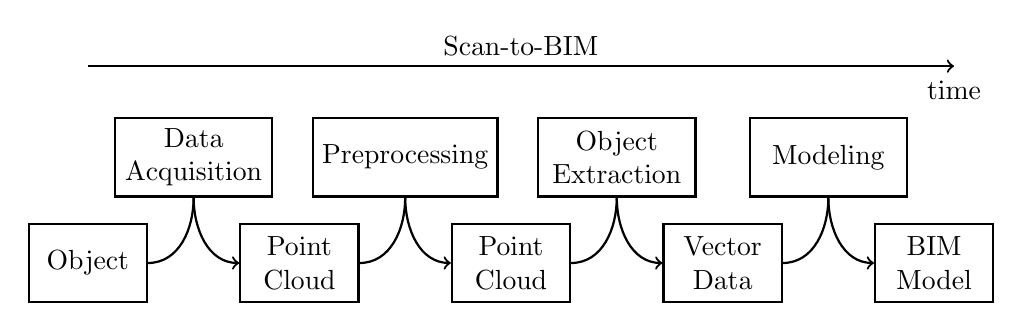
\begin{tikzpicture}[
        node distance=1.9cm, % Distance between nodes
        object/.style={draw, minimum width=1.5cm, minimum height=1cm, align=center}, % Box styling
        process/.style={draw, minimum width=2cm, minimum height=1cm, align=center}, % Box styling
        every path/.style={thick, -stealth} % Arrow styling
        ]
        
        % Define nodes
        \node (object) [object] {Object};
        \node (RC) [process, above right of=object] {Data \\ Acquisition};
        \node (pointcloud1) [object, below right of=RC] {Point \\ Cloud};
        \node (PP) [process, above right of=pointcloud1] {Preprocessing};
        \node (pointcloud2) [object, below right of=PP] {Point \\ Cloud};
        \node (Segmentation) [process, above right of=pointcloud2] {Object \\ Extraction};
        \node (vector) [object, below right of=Segmentation] {Vector \\ Data};
        \node (Modeling) [process, above right of=vector] {Modeling};
        \node (BIM) [object, below right of=Modeling] {BIM \\ Model};

        % Draw arrows
        \draw[-] (object.east) to[out=0, in=270] (RC.south);
        \draw[->] (RC.south) to[out=270, in=180] (pointcloud1.west);

        \draw[-] (pointcloud1.east) to[out=0, in=270] (PP.south);
        \draw[->] (PP.south) to[out=270, in=180] (pointcloud2.west);

        \draw[-] (pointcloud2.east) to[out=0, in=270] (Segmentation.south);
        \draw[->] (Segmentation.south) to[out=270, in=180] (vector.west);

        \draw[-] (vector.east) to[out=0, in=270] (Modeling.south);
        \draw[->] (Modeling.south) to[out=270, in=180] (BIM.west);
        
        % Draw Scan-to-BIM arrow
        \draw[->] (0,2.5) -- (11,2.5) node[midway, above] {Scan-to-BIM};
        \node at (11,2.2) {time}; 

    \end{tikzpicture}
    \caption{Derived Scan-to-BIM Workflow}
    \label {fig:Scan_to_BIM_workflow}
\end{figure}

\subsection{Data Acquisition}
\begin{German}
    Die Datenakquise erfolgt mittels Reality-Capture. Dabei wird ein physisches Objekt mithilfe von Sensoren digital erfasst und repräsentiert. Für Scan-to-BIM werden zwei Haupttechnologien verwendet \cite{rashdiScanningTechnologiesBuilding2022}:
    
    \begin{itemize}
        \item \textbf{Light Detection and Ranging (LiDAR):} LiDAR ist ein aktives, direktes Messverfahren zur Distanzbestimmung. Ein Emitter sendet Laserimpulse aus, die von Objekten reflektiert und von einem Detektor empfangen werden. Aus der gemessenen Laufzeit wird die Entfernung berechnet. Als natives Ausgabeformat wird direkt eine Punktwolke erzeugt. LiDAR-Scanner können nach gewählter Plattform in drei Kategorien unterteilt werden:
        \begin{enumerate}
            \item \textbf{Terrestrischer Laserscanner (TLS):} stationär auf einem Stativ, für präzise Umgebungserfassung.
            \item \textbf{Mobiler Laserscanner (MLS):} handgeführt, flexibel für enge oder schwer zugängliche Bereiche.
            \item \textbf{Airborne Laserscanner (ALS)} auf Drohnen montiert, ideal für Fassaden oder grössere Areale.
        \end{enumerate}
        \item \textbf{Photogrammetrie:} Photogrammetrie ist ein passives, indirektes Messverfahren, das auf der Auswertung überlappender Fotos aus verschiedenen Blickwinkeln basiert. Aus Bildgeometrie und Perspektivunterschieden können Punktwolken oder Meshes rekonstruiert werden.
    \end{itemize}

    LiDAR hat gegenüber Photogrammetrie eine meist höhere Genauigkeit und eignet sich ideal für die Erfassung von Innenräumen sowie bei schlechten Lichtverhältnissen. Photogrammetrie hingegen erfordert keine kostspielige Spezialhardware und stellt damit eine vergleichsweise kostengünstige Alternative dar. Sie wird häufig in Kombination mit Drohnen zur Erfassung von Außenfassaden eingesetzt \cite{rashdiScanningTechnologiesBuilding2022}.
    Als Ausgabeformat sind folgende beiden 3D-Repräsentationen verbeitet \cite{borrusoProceduralPointCloud2023,liu3DPointCloud2021}:

    \begin{itemize}
        \item \textbf{Punktwolke:} Eine Punktwolke ist eine Menge von Punkten im dreidimensionalen Raum. Jeder Punkt repräsentiert eine Oberflächenposition (x, y, z) des gescannten Objekts. Neben der Position können den Punkten weitere Attribute wie Farbwerte (r, g, b) oder ein Normalenvektor (nx, ny, nz) zugeordnet sein. Der Normalenvektor beschreibt die Ausrichtung der Oberfläche an der jeweiligen Punktposition und dient vielen Algorithmen als Inputparameter. Im Gegensatz zu Voxel-Grids, dem dreidimensionale Pendant zu einem 2D-Bild, haben die Punkte keine Gitterstruktur. Sie sind strukturfrei, was sie rechnerisch aufwendiger in der Verarbeitung macht. Punktwolken eignen sich besonders gut für präzise Analysen. 
        \item \textbf{Mesh:} Ein Mesh ist eine flächenhafte 3D-Repräsentation eines Objekts, die aus einer Menge von Eckpunkten (Vertices) sowie deren Verbindungen (Kanten und Flächen) besteht. Meist werden die Flächen als Dreiecke definiert, wodurch ein sogenanntes Dreiecksnetz entsteht. Meshes eignen sich besonders gut für realistische Visualisierungen.
    \end{itemize}

    Im weiteren Verlauf der Arbeit liegt der Fokus auf Punktwolken. Die zentralen Qualitätsmetriken hierfür sind \cite{rashdiScanningTechnologiesBuilding2022}:

    % Genauigkeit = Accuracy
    % Präzision = Precision
    % Punktdichte = Point Density
    % Auflösung = Resolution

    \begin{itemize}
        \item \textbf{Genauigkeit:} Beschreibt, wie genau die erfassten Punktpositionen (x, y, z) die tatsächliche Geometrie des realen Objekts widerspiegeln. Sie gibt also an, wie gross die Abweichung zwischen Messwert und wahrer Position ist.
        \item \textbf{Präzision:} Beschreibt die Wiederholgenauigkeit der Messung. Beschreibt somit, wie konsistent die einzelnen Punktpositionen erfasst werden, wenn dasselbe Objekt mehrfach unter denselben Bedingungen gemessen wird.
        \item \textbf{Punktdichte:} Beschreibt, wie viele Messpunkte in einer Punktwolke pro Flächeneinheit erfasst wurden. Sie ist ein Mass für die Detailauflösung der Punktwolke.
        \item \textbf{Auflösung:} Beschreibt den kleinsten räumlichen Abstand, den ein Sensorsystem beim Scannen unterscheiden oder erfassen kann. Sie bestimmt also, wie fein Details in der Punktwolke abgebildet werden können.
    \end{itemize}

\end{German}

\begin{English}
    Data acquisition is done using reality capture. A physical object is digitally captured and represented using sensors. Two main technologies are used for Scan-to-BIM \cite{rashdiScanningTechnologiesBuilding2022}:

    \begin{itemize}
        \item \textbf{Light Detection and Ranging (LiDAR):} LiDAR is an active, direct measurement method for distance determination. An emitter sends out laser pulses that are reflected by objects and received by a detector. The distance is calculated from the measured time of flight. A point cloud is directly generated as the native output format. LiDAR scanners can be divided into three categories depending on the chosen platform:
        \begin{enumerate}
            \item \textbf{Terrestrial LiDAR Scanner (TLS):} stationary on a tripod, for precise environment capture.
            \item \textbf{Mobile LiDAR Scanner (MLS):} handheld, flexible for tight or hard-to-reach areas.
            \item \textbf{Airborne LiDAR Scanner (ALS):} mounted on drones, ideal for facades or larger areas.
        \end{enumerate}
        \item \textbf{Photogrammetry:} Photogrammetry is a passive, indirect measurement method based on the evaluation of overlapping photos from different perspectives. Point clouds or meshes can be reconstructed from image geometry and perspective differences.
    \end{itemize}

    LiDAR usually has higher accuracy than photogrammetry and is ideal for capturing interiors and poor lighting conditions. Photogrammetry, on the other hand, does not require expensive special hardware and is therefore a relatively cost-effective alternative. It is often used in combination with drones for capturing exterior facades \cite{rashdiScanningTechnologiesBuilding2022}. The following two 3D representations are common output formats \cite{borrusoProceduralPointCloud2023,liu3DPointCloud2021}:

    \begin{itemize}
        \item \textbf{Point Cloud:} A point cloud is a set of points in three-dimensional space. Each point represents a surface position (x, y, z) of the scanned object. In addition to the position, the points can be assigned additional attributes such as color values (r, g, b) or a normal vector (nx, ny, nz). The normal vector describes the orientation of the surface at the respective point position and serves as an input parameter for many algorithms. Point clouds are particularly suitable for precise analyses.
        \item \textbf{Mesh:} A mesh is a planar 3D representation of an object consisting of a set of vertices and their connections (edges and faces). The faces are usually defined as triangles, creating a so-called triangle mesh. Meshes are particularly suitable for realistic visualizations.
    \end{itemize}

    The focus of this work is on point clouds. The central quality metrics for this are \cite{rashdiScanningTechnologiesBuilding2022}:

    \begin{itemize}
        \item \textbf{Accuracy:} Describes how accurately the captured point positions (x, y, z) reflect the actual geometry of the real object. It indicates how large the deviation between the measured value and the true position is.
        \item \textbf{Precision:} Describes the repeatability of the measurement. It describes how consistently the individual point positions are captured when the same object is measured multiple times under the same conditions.
        \item \textbf{Point Density:} Describes how many measurement points were captured in a point cloud per unit area. It is a measure of the detail resolution of the point cloud.
        \item \textbf{Resolution:} Describes the smallest spatial distance that a sensor system can distinguish or capture when scanning. It determines how fine details can be represented in the point cloud.
    \end{itemize}
\end{English}

% Kongruenztransformation = Rigid Transformation
% Grobregistrierung = Coarse Registration
% Feinregistrierung = Fine Registration

\subsection{Preprocessing}
\begin{German}
    Im \textbf{Preprocessing} wird die Punktwolke für weiterführende Analysen aufbereitet. Dabei können unter anderem folgende Schritte durchgeführt werden \cite{rashdiScanningTechnologiesBuilding2022,liu3DPointCloud2021}:
\end{German}

\begin{English}
    In the \textbf{Preprocessing} step, the point cloud is prepared for further analysis. The following steps can be performed \cite{rashdiScanningTechnologiesBuilding2022,liu3DPointCloud2021}:
\end{English}

\subsubsection{Registration}
\begin{German}
    Da dieser Schritt bei Photogrammetrie automatisch im Rahmen der Bündelblockausgleichung erfolgt, wird im Folgenden die Registrierung von LiDAR-Punktwolken betrachtet. Bei jedem Scanvorgang wird eine Punktwolke in seinem eigenen lokalen Koordinatensystem (SCS) erfasst. Um die Punktwolken in ein gemeinsames Koordinatensystem zu überführen, müssen die Punktwolken zueinander räumlich ausgerichtet werden. Dafür werden die lokalen Koordinatensysteme mittels einer Kongruenztransformation (Translation, Rotation) in ein lokales Koordinatensystem (LCS) überführt. Ziel ist es, eine zusammenhängende, vollständige Punktwolke zu erzeugen, in der alle Teilbereiche korrekt zueinander positioniert sind. Die Methoden können in zwei Kategorien unterteilt werden:

    \begin{enumerate}
        \item \textbf{Grobregistrierung:} Die Grobregistrierung ist der erste Schritt im Registrierungsprozess und dient der groben Ausrichtung zweier oder mehrerer Punktwolken, die sich in unterschiedlichen Koordinatensystemen befinden. Ziel ist es, eine annähernde Überlappung zu erzeugen, sodass eine nachfolgende Feinregistrierung möglich wird. Die Grobregistrierung kann manuell oder automatisiert erfolgen. Bei automatisierten Methoden werden beispielsweise charakteristische Merkmale in den Punktwolken erkannt und miteinander abgeglichen.
        \item \textbf{Feinregistrierung:} Die Feinregistrierung ist der zweite Schritt im Registrierungsprozess und verfeinert die grobe Ausrichtung, indem sie eine präzise Transformation zwischen überlappenden Bereichen der Punktwolken berechnet. Die Feinregistrierung erfolgt meist automatisiert und basiert häufig auf iterativen Algorithmen, die die Abweichung zwischen den Punktwolken minimieren.\\
        \textit{Beispiel: Iterative Closest Point (ICP)}
    \end{enumerate}
\end{German}

\begin{English}
    Since this step is done automatically in the context of bundle block adjustment in photogrammetry, the registration of LiDAR point clouds is considered below. In each scanning process, a point cloud is captured in its own local coordinate system (LCS). To transfer the point clouds to a common coordinate system, the point clouds must be spatially aligned with each other. For this purpose, the local coordinate systems are transformed into a local coordinate system (LCS) using a rigid transformation (translation, rotation). The aim is to create a coherent, complete point cloud in which all subareas are correctly positioned relative to each other. The methods can be divided into two categories:

    \begin{enumerate}
        \item \textbf{Coarse Registration:} Coarse registration is the first step in the registration process and serves to roughly align two or more point clouds that are in different coordinate systems. The aim is to create an approximate overlap so that subsequent fine registration is possible. Coarse registration can be done manually or automatically. In automated methods, for example, characteristic features in the point clouds are detected and matched with each other.
        \item \textbf{Fine Registration:} Fine registration is the second step in the registration process and refines the coarse alignment by calculating a precise transformation between overlapping areas of the point clouds. Fine registration is usually done automatically and is often based on iterative algorithms that minimize the deviation between the point clouds. \\
        \textit{Example: Iterative Closest Point (ICP)}
    \end{enumerate}
\end{English}

\subsubsection{Georeferencing}
\begin{German}
    Die Georeferenzierung ist der Prozess, bei dem eine Punktwolke aus einem lokalen Koordinatensystem (LCS) in ein übergeordnetes, globales Koordinatensystem (GCS) überführt wird. Ziel ist es, die Punktwolke räumlich korrekt in Bezug auf reale Weltkoordinaten zu verorten, sodass sie mit anderen Geodaten kombiniert und weiterverwendet werden kann. Für die Georeferenzierung werden häufig Referenzpunkte, s.g. Ground Control Points (GCPs), verwendet. Diese sind markante Punkte in der realen Welt, deren Koordinaten bekannt sind. Die Punktwolke wird dann über eine Helmert-Transformation (Translation, Rotation, Skalierung) in das GCS überführt. Die Genauigkeit der Georeferenzierung hängt von der Anzahl und Geometrie der GCPs ab. Je mehr GCPs verwendet werden, desto genauer ist die Transformation. \cite{voordendagKursGeodaetischeMesstechnik}
\end{German}

\begin{English}
    Georeferencing is the process of transferring a point cloud from a local coordinate system (LCS) to a higher-level, global coordinate system (GCS). The aim is to spatially locate the point cloud correctly in relation to real-world coordinates so that it can be combined and reused with other geodata. Georeferencing often uses reference points, so-called Ground Control Points (GCPs). These are distinctive points in the real world whose coordinates are known. The point cloud is then transformed into the GCS using a Helmert transformation (translation, rotation, scaling). The accuracy of the georeferencing depends on the number and geometry of the GCPs. The more GCPs are used, the more accurate the transformation. \cite{voordendagKursGeodaetischeMesstechnik}
\end{English}

\subsubsection{Filtering}
\begin{German}
    Punktwolken entahlten häufig unerwünschte Punkte, die die Qualität der Daten beeinträchtigen. Diese können beispielsweise durch Messrauschen, Ausreisser oder unerwünschte Objekte entstehen. Die Filterung dient dazu, die Punktwolke von solch unerwünschten Punkten zu bereiningen. Dabei können folgende Filter angewendet werden \cite{liu3DPointCloud2021}:

    \begin{enumerate}
        \item \textbf{Rauschfilter:} Rauschen bezeichnet zufällige, kleinräumige Abweichungen der Messpunkte von ihrer tatsächlichen Position. Es kann durch Sensorrauschen, ungünstige Oberflächeneigenschaften oder äussere Einflüsse wie Lichtverhältnisse entstehen. Um die Qualität der Punktwolke zu verbessern, werden Rauschfilter eingesetzt, die diese Abweichungen reduzieren oder betroffene Punkte entfernen.\\
        \textit{Beispiel: Moving Least Squares Filter (MLS)}
        
        \item \textbf{Ausreisserfilter:} Ausreisser sind einzelne Messpunkte, deren Lage signifikant von der sie umgebenden Punktverteilung abweicht und die nicht zur tatsächlichen Objektgeometrie gehören. Sie entstehen häufig durch Messfehler, Reflexionen oder Störungen während der Datenerfassung. Zur Verbesserung der Datenqualität werden Ausreisserfilter eingesetzt, die solche Punkte erkennen und entfernen.\\
        \textit{Beispiel: Statistical Outlier Removal Filter (SOR)}
    \end{enumerate}
\end{German}

\begin{English}
    Point clouds often contain unwanted points that affect the quality of the data. These can be caused by measurement noise, outliers, or unwanted objects. Filtering is used to clean the point cloud of such unwanted points. The following filters can be applied \cite{liu3DPointCloud2021}:

    \begin{enumerate}
        \item \textbf{Noise Filter:} Noise refers to random, small-scale deviations of the measurement points from their actual position. It can be caused by sensor noise, unfavorable surface properties, or external influences such as lighting conditions. Noise filters are used to improve the quality of the point cloud by reducing these deviations or removing affected points.\\
        \textit{Example: Moving Least Squares Filter (MLS)}
        
        \item \textbf{Outlier Filter:} Outliers are individual measurement points whose position significantly deviates from the surrounding point distribution and do not belong to the actual object geometry. They are often caused by measurement errors, reflections, or disturbances during data acquisition. Outlier filters are used to improve data quality by detecting and removing such points.\\
        \textit{Example: Statistical Outlier Removal Filter (SOR)}
    \end{enumerate}
\end{English}

\subsubsection{Downsampling}
\begin{German}
        Downsampling bezeichnet Verfahren zur gezielten Reduktion der Punktanzahl innerhalb einer Punktwolke. Die geometrisch wesentlichen Strukturen soll dabei erhalten bleiben. Ziel ist es, die Datenmenge zu verringern, um die Effizienz der anschliessenden Punktwolkenverarbeitung zu steigern.\\
        \textit{Beispiel: Voxel Grid Downsampling, Farthest Point Sampling (FPS), Normal Space Sampling (NSS)}
\end{German}

\begin{English}
    Downsampling refers to methods for selectively reducing the number of points within a point cloud. The geometrically essential structures should be preserved. The aim is to reduce the amount of data to increase the efficiency of subsequent point cloud processing.\\
    \textit{Example: Voxel Grid Downsampling, Farthest Point Sampling (FPS), Normal Space Sampling (NSS)}
\end{English}
  

\subsection{Segmentation}
\begin{German}
    Die \textbf{Segmentation} ist ein Prozess, bei dem die Punktwolke in einzelne Objekte oder Bauteile unterteilt wird. Dabei werden folgende Methoden unterschieden:

    \begin{enumerate}
        \item \textbf{Manuelle Segmentierung:} TODO: Beschreibung
        \item \textbf{Semi-automatische Segmentierung:} TODO: Beschreibung
        \item \textbf{Automatische Segmentierung:} TODO: Beschreibung
    \end{enumerate}
\end{German}

\begin{English}
    \textbf{Segmentation} is a process in which the point cloud is divided into individual objects or components. The following methods are distinguished:

    \begin{itemize}
        \item \textbf{Manual Segmentation:} TODO: Description
        \item \textbf{Semi-automatic Segmentation:} TODO: Description
        \item \textbf{Automatic Segmentation:} TODO: Description
    \end{itemize}
\end{English}

\subsection{Modeling}
\begin{German}
    Der \textbf{Modeling}-Schritt dient dazu, die Vektor-Daten aus der Punktwolke in ein BIM-Modell zu überführen. Dabei werden folgende Methoden unterschieden:

    \begin{enumerate}
        \item \textbf{Manuelles Modellieren:} TODO: Beschreibung
        \item \textbf{Semi-automatisches Modellieren:} TODO: Beschreibung
        \item \textbf{Automatisches Modellieren:} TODO: Beschreibung
    \end{enumerate}
\end{German}

\begin{English}
    The \textbf{Modeling} step is used to transfer the vector data from the point cloud into a BIM model. The following methods are distinguished:

    \begin{itemize}
        \item \textbf{Manual Modeling:} TODO: Description
        \item \textbf{Semi-automatic Modeling:} TODO: Description
        \item \textbf{Automatic Modeling:} TODO: Description
    \end{itemize}
\end{English}